%\documentclass[aspectratio=169, handout]{beamer}
\documentclass[aspectratio=169]{beamer}


\makeatletter
\renewcommand*\env@matrix[1][\arraystretch]{%
  \edef\arraystretch{#1}%
  \hskip -\arraycolsep
  \let\@ifnextchar\new@ifnextchar
  \array{*\c@MaxMatrixCols c}}
\makeatother

\usepackage{tikz}
\usetikzlibrary{tikzmark,fit,shapes.geometric}


\newcommand{\transp}{^{\rm{T}}}

\usepackage{cases}
\usepackage[english]{babel}
% or whatever
\usepackage{xcolor}
\usepackage{colortbl}
\usepackage[latin1]{inputenc}
\usepackage[super]{nth}
% or whatever
%\setbeamertemplate{footline}[page number]
\setbeamertemplate{footline}
        {
      \leavevmode%
      \hbox{%
      \begin{beamercolorbox}[wd=.333333\paperwidth,ht=2.25ex,dp=1ex,center]{author in head/foot}%
        \usebeamerfont{author in head/foot}\insertshortauthor%~~(\insertshortinstitute)
      \end{beamercolorbox}%
      \begin{beamercolorbox}[wd=.333333\paperwidth,ht=2.25ex,dp=1ex,center]{title in head/foot}%
        \usebeamerfont{title in head/foot}\insertshorttitle
      \end{beamercolorbox}%
      \begin{beamercolorbox}[wd=.333333\paperwidth,ht=2.25ex,dp=1ex,right]{date in head/foot}%
        \usebeamerfont{date in head/foot}\insertshortdate{}\hspace*{2em} \insertframenumber{}  \hspace*{2em}%/ \inserttotalframenumber\hspace*{2ex} 

    %#turning the next line into a comment, erases the frame numbers
        

      \end{beamercolorbox}}%
      \vskip 0pt%
    }

\usepackage{times}
\usepackage[T1]{fontenc}
\usepackage{psfrag}
\usepackage{algorithm}
\usepackage{amsmath}
\usepackage{amssymb}
\usepackage{tabularx}
\usepackage{algpseudocode}
\usepackage{mathrsfs}
\usepackage{textpos}
\usepackage{graphicx}
\usepackage{tcolorbox}
\usepackage{multicol}
\usepackage{tikz}
\usetikzlibrary{arrows.meta,shapes.arrows}
%\setkeys{Gin}{draft}
\usepackage{caption}
\captionsetup{font=scriptsize,labelfont=scriptsize}
\usepackage{color}
\DeclareCaptionFont{blue}{\color{blue}}
\captionsetup{labelfont=blue}
\usepackage{tikz}
\tikzset{
  every overlay node/.style={
    draw=white,anchor=north west,
  },
}
\def\checkmark{\tikz\fill[scale=0.4](0,.35) -- (.25,0) -- (1,.7) -- (.25,.15) -- cycle;}
\def\tikzoverlay{%
   \tikz[baseline,overlay]\node[every overlay node]
}%
%\DeclareGraphicsRule{.png}{png}{.png.bb}{}

\newtheorem{assumption}{Assumption} %jw

\newcommand{\T}{{\rm T}}

\newcommand\blfootnote[1]{%
  \begingroup
  \renewcommand\thefootnote{}\footnote{#1}%
  \addtocounter{footnote}{-1}%
  \endgroup
}
\setcounter{tocdepth}{1}
\beamertemplatenavigationsymbolsempty


\title[Lecture 13: Gradient Descent] % (optional, use only with long paper titles)
{Data, Environment and Society: \\{Lecture 13: Gradient Descent}}


%\subtitle
%{Include Only If Paper Has a Subtitle}

\author[ER190C: Data, Environment and Society] 
{Instructor: Duncan Callaway\\
GSI: Seigi Karasaki} 
% - Give the names in the same order as the appear in the paper.
% - Use the \inst{?} command only if the authors have different
%   affiliation.

%\logo{
%\includegraphics[width=1.5cm,height=1.5cm,keepaspectratio]{uvic_logo_h.jpg}
%}
\vspace{-20mm}
\institute[UC Berkeley] % (optional, but mostly needed)
 {\small{ \bf October 4, 2018}}


\date[October 4, 2018]


\begin{document}

\begin{frame}[plain, noframenumbering]
  \titlepage
\end{frame}

\begin{frame}{Announcements}

\textbf{Today}
\begin{itemize}
\item Gradient descent
\item Environmental Justice
\end{itemize}

\textbf{Reading}
\begin{itemize}
\item Today: Ch 11 DS100
\item Next \textit{thursday:} Clark \textit{et al} (using LUR data for EJ questions)
\end{itemize}
\end{frame}


\begin{frame}{Survey results}
\begin{figure}
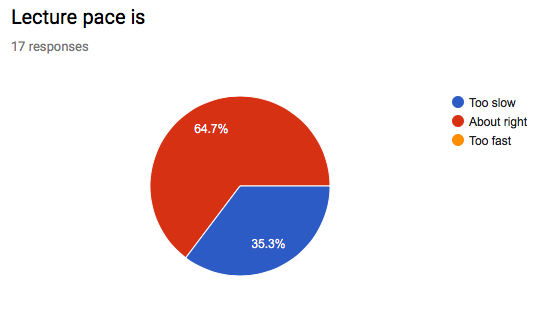
\includegraphics[width=\textwidth]{survey_pace}
\caption*{}
\end{figure}
\end{frame}

\begin{frame}{Survey results}
\begin{figure}
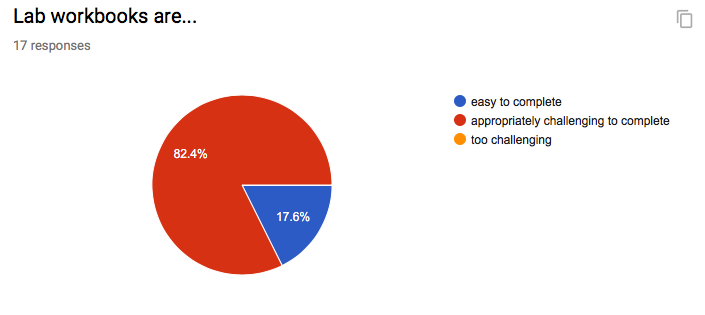
\includegraphics[width=\textwidth]{survey_lab_notebooks}
\caption*{}
\end{figure}
\end{frame}

\begin{frame}{Survey results}
\begin{figure}
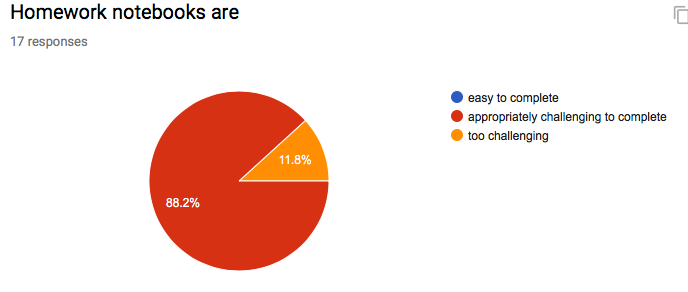
\includegraphics[width=\textwidth]{survey_hw}
\caption*{}
\end{figure}
\end{frame}

\begin{frame}{Survey results}
\begin{figure}
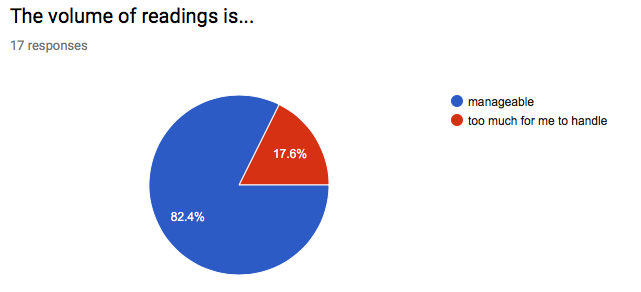
\includegraphics[width=\textwidth]{survey_readings}
\caption*{}
\end{figure}
\end{frame}

\begin{frame}{Survey results: A few key takeaways}


\begin{itemize}
\item Students asked for more time for discussion and interaction
\begin{itemize}
\item<2-> Will work to make this change
\end{itemize}
\item A few students suggested I assume background reading is done...
\begin{itemize}
\item<3-> I'm trying to do this, then reinforcing what I feel are key points from ISLR.
\end{itemize}
\item Request for more board work
\begin{itemize}
\item<4-> I will work to do more on the iPad -- is that working?
\end{itemize}
\item Requests for more energy-enviro applications
\begin{itemize}
\item<5-> Trying!  Also need to make sure we cover methods...but we'll try to get more in.
\end{itemize}
\item Students are struggling to find a way to take notes
\begin{itemize}
\item<6-> Any suggestions?
\end{itemize}
\item Grading rubric, more clarity on questions in HW and Labs
\begin{itemize}
\item<7-> We may not get a rubric, but we will work to clarify and ensure fair grading
\end{itemize}
\item Lots of positive feedback for Seigi
\begin{itemize}
\item<8-> Your GSI rocks!
\end{itemize}
\end{itemize}
\end{frame}

\begin{frame}{Basic estimation process, so far}
\begin{enumerate}
\item Define a loss function
\item Set derivatives of loss function equal to zero and solve for parameters
\end{enumerate}

\vspace{5mm}
The challenge:
\begin{itemize}
\item Setting loss function derivatives to zero not always easy.
\item This doesn't scale well for big problems (e.g. many different nonlinear transformations of the Novotny data)
\end{itemize}
\end{frame}

\begin{frame}{The loss function}

Mean squared error, aka the `L2' norm
\uncover<2->{
	\begin{align*}
		\text{MSE} &= \frac{1}{n}\sum_{i=1}^n (y_i - \hat{y}_i)^2\\
		\text{Constant model,} \hat{y} = \theta \rightarrow \text{MSE} &= \frac{1}{n}\sum_{i=1}^n (y_i - {\theta})^2\\
	\end{align*}
}
Mean absolute error, aka the `L1' norm
\uncover<2->{
	\begin{align*}
		\text{MAE} &= \frac{1}{n}\sum_{i=1}^n |y_i - \hat{y}_i|\\
		&= \frac{1}{n}\sum_{i=1}^n |y_i - {\theta}|
	\end{align*}
}

\end{frame}

\begin{frame}{Advantages and disadvantages to MAE and MSE?}
\begin{figure}
	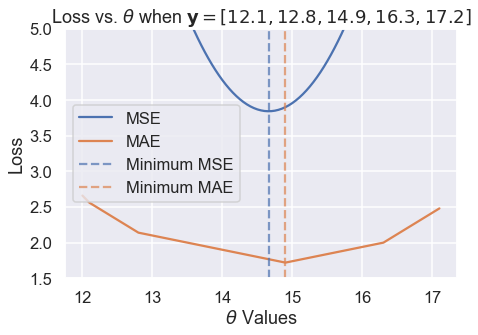
\includegraphics[width=0.5\textwidth]{mae_vs_mse}
	\caption*{}
\end{figure}
\pause
\vspace{-10mm}
\begin{itemize}
	\item MSE is differentiable $\rightarrow$ can solve directly for coefficients
	\item MAE is less impacted by extreme values
\end{itemize}
\end{frame}

\begin{frame}{Aside: what do these cost functions provide with the ``constant'' model?}

What well-known values minimize these loss functions?

	\begin{align*}
		\theta^*_{\text{MSE}} = \arg \min_\theta  \frac{1}{n}\sum_{i=1}^n (y_i - \theta)^2\\
		\theta^*_{\text{MAE}} = \arg \min_\theta  \frac{1}{n}\sum_{i=1}^n |y_i - \theta|
	\end{align*}
\pause
\begin{itemize}
	\item MSE returns the mean value of a sequence
	\item MAE returns the \textit{median}
\end{itemize}

\end{frame}

\begin{frame}{Huber loss}

\begin{columns}
\column{0.6\textwidth}
\begin{figure}
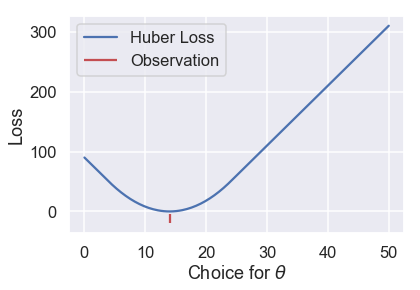
\includegraphics[width=0.85\textwidth]{huber}
\caption*{}
\end{figure}
\vspace{-10mm}
\begin{align*}
L_\delta(\theta, \textbf{y}) = \frac{1}{n} \sum_{i=1}^n 
\begin{cases}
    \frac{1}{2}(y_i - \theta)^2 &  | y_i - \theta | \le \delta \\
    \delta ( |y_i - \theta| - \frac{1}{2}\delta ) & \text{otherwise}
\end{cases}
\end{align*}
\column{0.4\textwidth}
What does this buy us?
\pause
\begin{itemize}
\item Differentiable
\item Absolute value at extremes -- not dominated by outlier.
\end{itemize}

\vspace{5mm}
\pause
What does this cost us?
\pause
\begin{itemize}
\item Optimal solution requires derivative w.r.t. $\theta$ \textit{and} derivative w.r.t. $\delta$ equal zero.  
\item That can be tricky.
\end{itemize}
\end{columns}
\end{frame}

\begin{frame}{Estimation takeaway \# 1: }

Analytical solutions for parameters (e.g. by setting partial derivatives equal to zero) not always available for some of the types of loss functions we'd like to use.
\end{frame}

\begin{frame}{Estimation takeaway \# 2: }

A separate issue: In situations where the normal equations (or something like them) can be used to solve for parameters:

\begin{align*}
\Theta &=  
(X^TX)^{-1}X^TY
\end{align*}

It can be very difficult computationally to invert a large $X^TX$ (I crashed my computer with 50,000 by 50,000).  
\end{frame}



\begin{frame}{Gradient descent -- sketch}

\pause
\begin{figure}
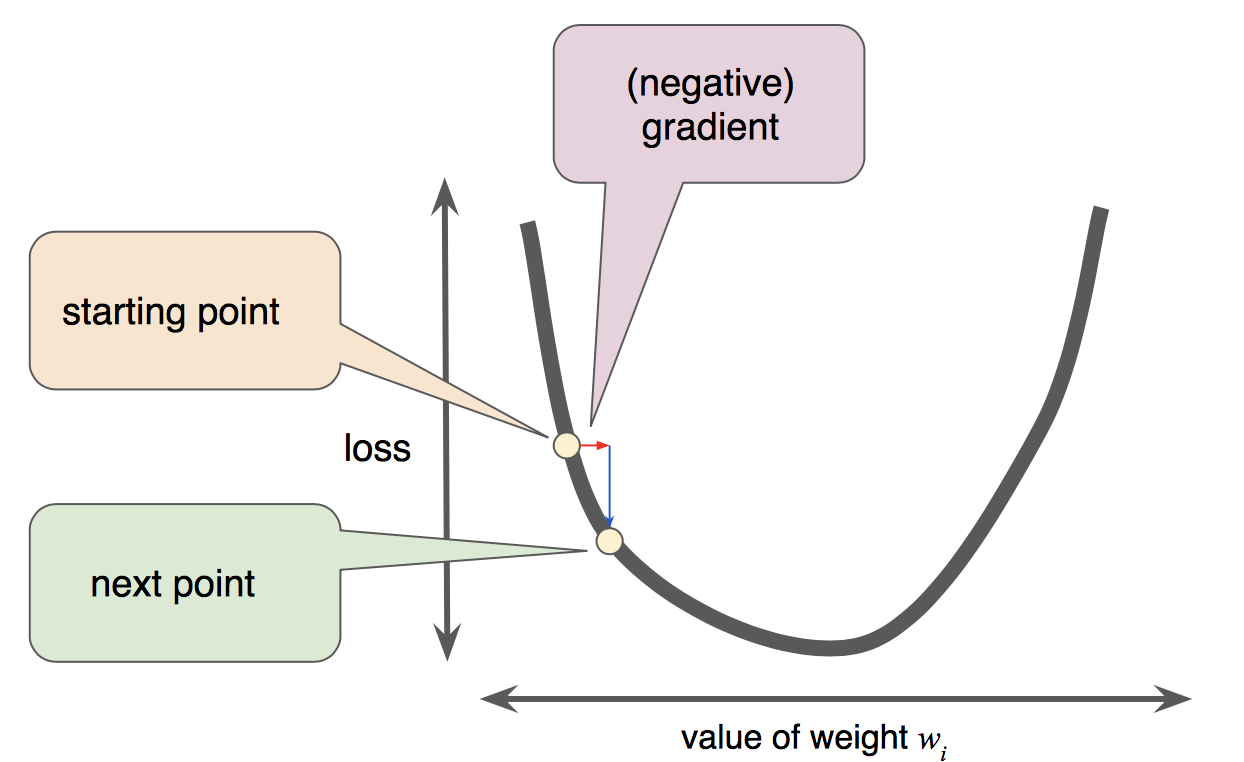
\includegraphics[height=0.7\textheight]{grad_desc_google_4}
\caption*{\url{https://developers.google.com/machine-learning/crash-course/reducing-loss/gradient-descent}}
\end{figure}

\end{frame}



\begin{frame}{Gradient descent -- math}

What's the gradient?  For our purposes, it is the slope of the loss function at a given point \textit{with respect to a particular parameter.}

\vspace{5mm}

The gradient is $\nabla_\theta L(\theta, \textbf{y}) = \uncover<2->{\frac{\partial}{\partial \theta} L(\theta, \textbf{y}).}$

\vspace{5mm}

\textbf{Gradient descent process}:
\begin{enumerate}
\item Choose a value for the ``learning rate'', $\alpha$
\item Choose a starting value of  $\theta$ (0 is a common choice).
\item Compute  $\theta - \alpha \cdot \frac{\partial}{\partial \theta} L(\theta, \textbf{y})$ and store this as the new value of $\theta$.  
\item Repeat until $\theta$ doesn't change (much) between iterations.
\end{enumerate}

\vspace{5mm}

\end{frame}

\begin{frame}{Gradient descent for quadratic loss}

\begin{columns}
\column{0.5\textwidth}
Let's derive the gradient:
\pause
\uncover<2->{
\begin{align*}
L &= \sum_{i=1}^n (y_i-\theta)^2\\
\frac{\partial L}{\partial \theta} & =  -2\sum_{i=1}^n (y_i-\theta)
\end{align*}
}
\column{0.5\textwidth}
...and then write a few iterations: 
\uncover<3->{\begin{align*}
\Rightarrow & \theta_1=0\\
					&\theta_2 = \theta_1 - \alpha(-2\sum_{i=1}^n (y_i-\theta_1))\\
					&\vdots\\
					&\theta_{t+1} = \theta_t - \alpha(-2\sum_{i=1}^n (y_i-\theta_t))
\end{align*}
Stop when $|\theta_{t+1} - \theta_t| < \text{tol}$, where ``tol'' is a small tolerance parameter.}
\end{columns}
\end{frame}

\begin{frame}{Gradient descent, in code}

%
%In other words:
%
%\vspace{5mm}
%
%$\theta^{(t+1)} = \theta^{(t)} - \alpha \cdot \nabla_\theta L(\theta^{(t)}, \textbf{y})$

\begin{figure}
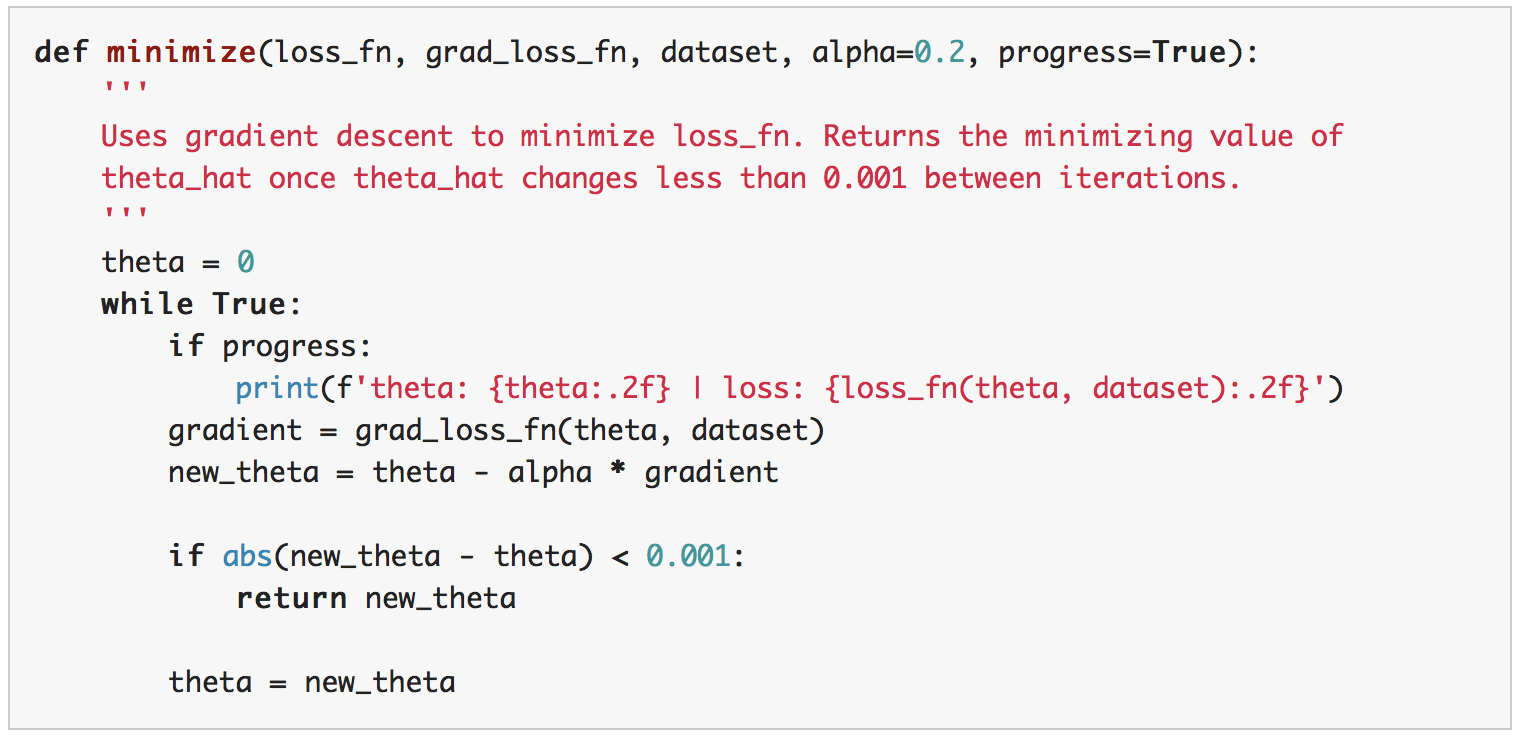
\includegraphics[width=1.\textwidth]{grad_desc}
\caption*{\url{https://www.textbook.ds100.org/ch/11/gradient_descent_define.html}}
\end{figure}

\end{frame}

\begin{frame}{Gradient descent -- what does the learning rate do?}

Get in small groups and play with this Google tool: \href{https://goo.gl/JNPhUv}{https://goo.gl/JNPhUv}.

\vspace{5mm}

Set $\alpha$ to a higher value than the default -- it'll take forever at $\alpha = 0.01$.  
\vspace{5mm}

Questions to answer together:  How does the rate change on each iteration...
\begin{enumerate}
\item ...when the learning rate is really small?
\item ...when the learning rate is really big?
\end{enumerate}


\pause
\vspace{5mm}
There are four qualitatively different behaviors:
\begin{enumerate}
\item Monotonically decreasing loss
\item One step to optimal parameter
\item Loss declines in periodic oscillations
\item Loss grows out of control
\end{enumerate}

\end{frame}

\begin{frame}{What do you think the point of a ``dynamic learning rate" might be?}

\pause

Basic idea: Start with a big learning rate, then make it smaller and smaller as you approach the optimal value

\pause

\vspace{10mm}

Advantages: 
\begin{itemize}
\item cover a lot of ground when you're far from the optimal value
\item refined steps when you get close, so you don't miss the optimal value.
\end{itemize}

\end{frame}

\begin{frame}{Absolute deviation loss, revisited}

\begin{columns}
\column{0.6\textwidth}
\begin{align*}
L &= \frac{1}{n} \sum_{i = 1}^{n}|y_i - \theta|\\
&= \frac{1}{n} \left( \sum_{y_i < \theta}|y_i - \theta| + \sum_{y_i = \theta}|y_i - \theta| + \sum_{y_i > \theta}|y_i - \theta| \right)\\
\frac{\partial L}{\partial \theta} &= \frac{1}{n} \left( \sum_{y_i < \theta}(-1) + \sum_{y_i = \theta}(0) + \sum_{y_i > \theta}(1) \right)
\end{align*}
\column{0.4\textwidth}
Can you see why the optimal value is the median?

\vspace{5mm}

\pause

The right solution just ``counts'' the number of observations on each side of the optimal value

\end{columns}

\end{frame}


\begin{frame}{Gradient descent -- absolute deviation loss, ctd.}

\begin{columns}
\column{0.5\textwidth}
	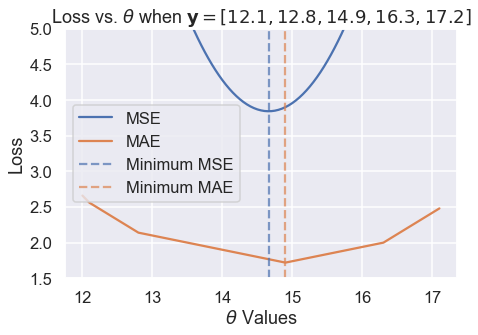
\includegraphics[width=\textwidth]{mae_vs_mse}

\column{0.5\textwidth}

What's the problem with doing gradient descent here?

\vspace{5mm}

\pause

The derivative does not go to zero at the optimal value.  

\vspace{5mm}

So once the solution is close, it won't converge, unless...\pause we use a dynamic learning rate.
\end{columns}

\end{frame}

\end{document}


